% TODO [ ] Increase font size to avoid migraines and Health and Safety issues for prospective employers.
\documentclass[9pt]{developercv}

% Allows us to insert an existing PDF into the document
\usepackage{pdfpages}
%----------------------------------------------------------------------------------------

\begin{document}

%----------------------------------------------------------------------------------------
%   TITLE AND CONTACT INFORMATION
%----------------------------------------------------------------------------------------

\begin{minipage}[t]{0.45\textwidth}
    \vspace{-\baselineskip}
    \colorbox{black}{{\HUGE\textcolor{white}{\textbf{\MakeUppercase{Jesse}}}}} % First name

    \colorbox{black}{{\HUGE\textcolor{white}{\textbf{\MakeUppercase{Wood}}}}} % Last name

    \vspace{6pt}

    {\huge Software Developer}
\end{minipage}
\begin{minipage}[t]{0.275\textwidth}
    \vspace{-\baselineskip}
    \icon{MapMarker}{12}{Wellington, New Zealand}\\
    \icon{Phone}{12}{+64 210 26 48190}\\
    \icon{At}{12}{\href{mailto:j.r.h.wood98@gmail.com}{j.r.h.wood98@gmail.com}}\\
\end{minipage}
\begin{minipage}[t]{0.275\textwidth}
    \vspace{-\baselineskip}
    \icon{Globe}{12}{\href{https://woodrock.github.io}{woodrock.github.io}}\\
    \icon{Github}{12}{\href{https://github.com/woodrock}{github.com/woodrock}}\\
    \icon{Linkedin}{12}{\href{https://www.linkedin.com/in/jrhwood/}{linkedin.com/in/jrhwood}}\\
\end{minipage}

\vspace{0.5cm}

%----------------------------------------------------------------------------------------
%   INTRODUCTION, SKILLS AND TECHNOLOGIES
%----------------------------------------------------------------------------------------
% TODO [x] Talk about what I have done specifically
% TODO [x] Don't frame me as a student
% TODO [x] Should highlight that there is gold here
% TODO [x] Specify which field, and areas of software engineering I am passionate about
% TODO [x] Work at Niwa is gold as are my hobbies in AI and Robotics
\cvsect{Personal Statement}

My goal is to leave the world a better place than I found it. I plan to bring that goal into reality by creating technology that improves the quality of life. These goals have motivated my passion for software engineering and the open-source community as a tool for sharing knowledge. This objective has led me an internship at NIWA, collaborating with scientists and physicists to publish their research on our oceans and atmosphere to a global audience. Software is a medium to explore my scientific curiosity and contribute a meaningful change.

%----------------------------------------------------------------------------------------
%   EXPERIENCE
%----------------------------------------------------------------------------------------
% TODO [x] merge bartending roles into a few transferrable skills
% TODO [x] serving customers to deliver their needs, conflict resolution skills and negotiation
% TODO [x] don't reduce the bartending wordcount, increase the gold

\cvsect{Experience}

\textbf{300 Level Tutoring} - 2021 to Present - \emph{\href{https://www.wgtn.ac.nz/}{Victoria University of Wellington}} , Wellington, NZ
\begin{itemize}
    \item Following the state of the art Human-Computer Interaction literature and Mobile Application Development frameworks covered in the course.
    \item Deliver tutorials to third-year students on how to develop mobile applications using modern JavaScript frameworks (i.e Ionic and React Native). 
    \item Marking and providing meaningful feedback on technical writing and implementations for mobile applications.
\end{itemize}

\textbf{Web and Content Intern} - 2021 to Present - \emph{\href{https://www.wecc.org.nz/}{Wellington Chamber of Commerce}} , Wellington, NZ
\begin{itemize}
    \item A strong focus on business and legislation helped develop the toolkit and familiarity with the knowledge and skills required to run a successful business.
    \item Data visualization to deliver engaging and interactive tools to explore business and marketing analysis data in a digitized form. 
    \item Web development using the iMIS Engagement Management System. Maintaining and developing new components that are dynamically generated from a database. 
    \item Collaboration with marketing and design teams using an agile methodology to deliver effective products that meet user requirements.
    % \item Presentations and technical documentation to communicate the development process and facilitate future work easily.
    % \item Working-remotely due to the renewed COVID-19 lockdowns. Utilizing industry-standard tools (i.e, Microsoft Teams, Microsoft Sharepoint and Github Projects)
\end{itemize}

\textbf{Software Intern} - 2020 to Present - \emph{\href{https://niwa.co.nz/}{NIWA}} , Wellington, NZ
\begin{itemize}
    \item Multi-disciplinary collaboration to implement an end to end best practice OGC Standard software.
    \item Open-source technology stack to create web services that queried a database on a Linux cloud server.
    \item Without previous expertise in Geo-Physics or Biology, Data Understanding was an important area of this work. We extracted requirements for software using the knowledge provided from other disciplines.
    \item Participate in weekly meetings to communicate progress. Documentation of work to non-technical users through best practise agile methodology.
    \item Work remotely from home due to the COVID-19 pandemic. Utilizing industry-standard tools (i.e, Microsoft Teams for communication and Pulse Secure for SSH).
\end{itemize}

\textbf{Front of House} - 2018 to 2019 - \emph{\href{https://stjohnsbar.co.nz/}{St. Johns Bar and Eatery}}, Wellington, NZ
\begin{itemize}
    \item Upsell new products or promotions.
    \item Organise a team to work efficiently.
    \item Deliver value to a customer and to be honest regarding roadblocks.
\end{itemize}

\textbf{Back of House / Front of House} - 2012 to 2018 - \emph{\href{https://macsbrewbar.co.nz/}{Mac's Brewery}}, Wellington, NZ
\begin{itemize}
    \item Upskilling to learn all aspects of the trade.
    \item Cope under pressure in a fast-paced work environment that involved risk management, i.e. negotiations with disorderly customers.
    \item Empathetic and Active Listening when dealing with confrontations.
\end{itemize}

%----------------------------------------------------------------------------------------
%   EDUCATION
%----------------------------------------------------------------------------------------
% TODO [x] include subjects with grades
% TODO [x] Expand on public speaking/debating
% TODO [ ] Include ENGR 201, Technical Writing paper which includes presentations, public speaking and report writing

\cvsect{Education}

\textbf{Bachelor of Engineering (Software Engineering)} - 2016 to Present - \emph{\href{https://www.wgtn.ac.nz/}{Victoria University of Wellington}}
\begin{itemize}
    \item Subjects were chosen to provide an academic background to supplement a full-stack developer. \textbf{Industry Research Project, Human-Computer Interaction, Deep Neural Networks, Compiler Engineering}
    \item \textbf{Class representative} for SWEN430 Compiler Engineering, liaison between students and faculty for course-related problems. 
    \item Volunteer position communicating information to make the university accessible to a wider audience. \textbf{Note-Taker}
    \item Awarded to those who excelled in their secondary school studies. \textbf{Victoria Excellence Scholarship}
\end{itemize}
\emph{N.B The Head of School's commentary on my grades is attached to this document.} \\

\textbf{NCEA Level 3} - 2011 to 2015 - \emph{Rongotai College}
\begin{itemize}
    \item These subjects provided the bedrock for a passion in Computer Science. \textbf{Computers, Physics, Calculus, English, Graphics, Music}
    \item Extra-curricular roles helped develop hone in public speaking and presentation skills. \textbf{Prefect, UN Youth Ambassador, Jazz Band, Production Band, Debating}
    \item This is an award for university level written communications skills given to secondary school students. \textbf{Scholarship English}
\end{itemize}

%----------------------------------------------------------------------------------------
%   ProjectsThe Wellington Hub was hosted by Niwa.
%----------------------------------------------------------------------------------------
% TODO [x] expand on project descriptions
% TODO [x] make descriptions generic to a subject matter, less focussed on technologies

\cvsect{Projects}

\textbf{Resource Portal} \\
The iMIS EMS is an Engagement Management System the Wellington Chamber of Commerce uses to manage the content on its website. I developed an automated workflow to digitize paper-based documents and to create a digital version of the documents. These documents were converted into responsive and engaging web pages. \\

\textbf{\href{https://github.com/woodRock/verbose-computing-machine}{Advent of Code}} \\
An advent calendar of programming puzzles that are language agnostic. The functional programming language Haskell was chosen. In Haskell, programs cannot store state so functions cannot have unintended side effects. Reducing the likelihood of errors meant solving problems faster. Incorrect submissions were penalized, so test cases were verified before submitting a final answer. \\

\textbf{\href{https://github.com/woodRock/psychic-invention}{Data Ingestion}} \\
Ingesting Benthic Biodiversity data into the \href{https://nzodn.nz/}{NZODN portal}. This is an open-source technology stack that implements OGC standards. It uses tools such as GeoServer to providing web services to display maps, and GeoNetwork as a CMS for a metadata catalogue. We configure the software to use a Postgres database storing geospatial data. \\

\textbf{Mission Control System} \\
Runs on a laptop in the field to display telemetry data from a rocket. It presents Monte Carlo simulation data to predict possible landing locations. It was developed as a group using agile and scrum methodologies. We strived for the software quality attribute of portability. To do this we implemented an open-source web map service that can display locally stored map data for offline usage.

%----------------------------------------------------------------------------------------
%   Technical Skills
%----------------------------------------------------------------------------------------
% TODO [x] mention areas of knowledge - Python, JavaScript, R, Git, LaTeX, Postgres
% TODO [x] avoid abstract measurements of capability. I am a student I don't have much experience in anything

\cvsect{Technical Tools}

\textbf{Scripting:} General knowledge of the fundamental principles and tradeoffs for a breadth and depth of programming languages. Consisting of both the Functional and Object Oriented paradigms, and a mix of High and Low-level languages. \textbf{JavaScript, HTML5, CSS, React, Angular, Vue, Java, Ruby, Haskell, Common-Lisp, C, C++} \\

\textbf{Machine Learning:} Practical experience implementing machine learning pipelines to produce business knowledge from real-world datasets. Use of scripting languages for preprocessing, exploratory data analysis, training and testing, and data visualization. \textbf{Python, Scikit-learn, TensorFlow, Keras, R, Weka} \\

\textbf{Databases:} Academic and practical knowledge in both SQL and NoSQL database systems. Created databases using cloud services that are utilized in full-stack applications. \textbf{Firebase, Postgres, iMIS, Postgis, SQLite, MongoDB} \\

\textbf{Workflow:} Git is an amazing tool for version control and agile documentation of development. It provides an excellent environment for a development community, working together asynchronously and remotely. \textbf{Git, Gitlab, Github, GitBucket, Jira, LaTeX, Markdown, PlantUML} \\

%----------------------------------------------------------------------------------------
%   Workshops
%----------------------------------------------------------------------------------------
% TODO [x] mention workshops  attended - Foss4G, Python Data Ingestion, Databases 101
\newpage
\cvsect{Workshops and Conferences}

\textbf{WOSSAT} \\ 
The Wellington Open Source Show and Tell (WOSSAT) is a monthly meetup hosted by Catalyst. This meetup demonstrates notable new technologies, hobby projects and open source advocacy. The open-source community promotes open standards and open data that reduce the barriers to access to technology. \\

\textbf{FOSS4G SoTM} \\
Due to the virus, local hubs for the international event were held. This conference covers cutting edge open-source GIS software. A former developer at MapBox found out their software was being used for drone strikes in the middle east. An important takeaway from the conference was the ethics of the software we develop. \\

\textbf{Python Data Ingestion} \\
The attendees were mostly data scientists and software developers. This covered using Python for Scientific Computing. We explored the Anaconda environment for Python development for package management. It can be used to replicate a python environment on another machine. A Jupyter notebook is an important tool for Literate Programming as it merges documentation and codebases. \\

\textbf{Databases 101} \\
There was an interesting discussion that compared RDBMS vs NoSQL databases. There is are certain tradeoffs between different software quality attributes, and risks involve getting vendor locked into proprietary cloud software (i.e., AWS, Azure or Firebase). As a developer who creates and maintains these databases, it was useful to understand the goals of the end-users of the product.

% ----------------------------------------------------------------------------------------
%   Hobbies
% ----------------------------------------------------------------------------------------

\cvsect{Hobbies}

% TODO [x] Move hobbies to the second page of the CV

{
  \textbf{Debating} \\
  Public speaking, politics, philosophy, UN Youth Ambassador\\
}
{
  \textbf{Sciences} \\
  CS, AI, Robotics, Astrophysics, Psychology \\
}
{
  \textbf{Guitar} \\
  Classical, Jazz, Blues, Classic Rock \\
}
{
  \textbf{Sports} \\
  Canoe Polo, Table Tennis
}

%----------------------------------------------------------------------------------------
%   References
%----------------------------------------------------------------------------------------


% TODO [x] Contact information for references is available upon request
% TODO [x] Reflect on data security and data privacy and ask what broadcasting contact information says to an employer
% TODO [x] Contact A University Tutor - Miru
% TODO [x] include titles/positions for each of the references
% TODO [x] connect to a soft skill for non-IT connections
% TODO [ ] Get a list of 10 and cater references for each job

\cvsect{References}

\textbf{Andrea Mari} - Research Software Engineer at \emph{Niwa} \\
Andrea is my mentor at Niwa. He has introduced me to the software development processes at Niwa, including Jira and regular agile meetings. I am humbled to learn from his industry expertise as a software developer.\\

\textbf{Tom Moorhead} - Functions Coordinator at \emph{Mac's Function Center} \\
We planned large scale events for several hundred people. We employed industry standards in catering and collaborated with the host to meet their vision for the event. \\

\textbf{Miniruwani Samrakoon} - Co-President, Postgraduate, Students Association at \emph{Victoria University} \\
Miniruwani was my tutor for my 300 level Engineering group project. This involved collaboration using agile methodologies to develop a web application. That application provided a Mission Control interface for a Rocket. \\

\emph{N.B Contact information is available upon request.}

%----------------------------------------------------------------------------------------
%   Academic Letter
%----------------------------------------------------------------------------------------
% TODO [x] Include academic letter from Head of School

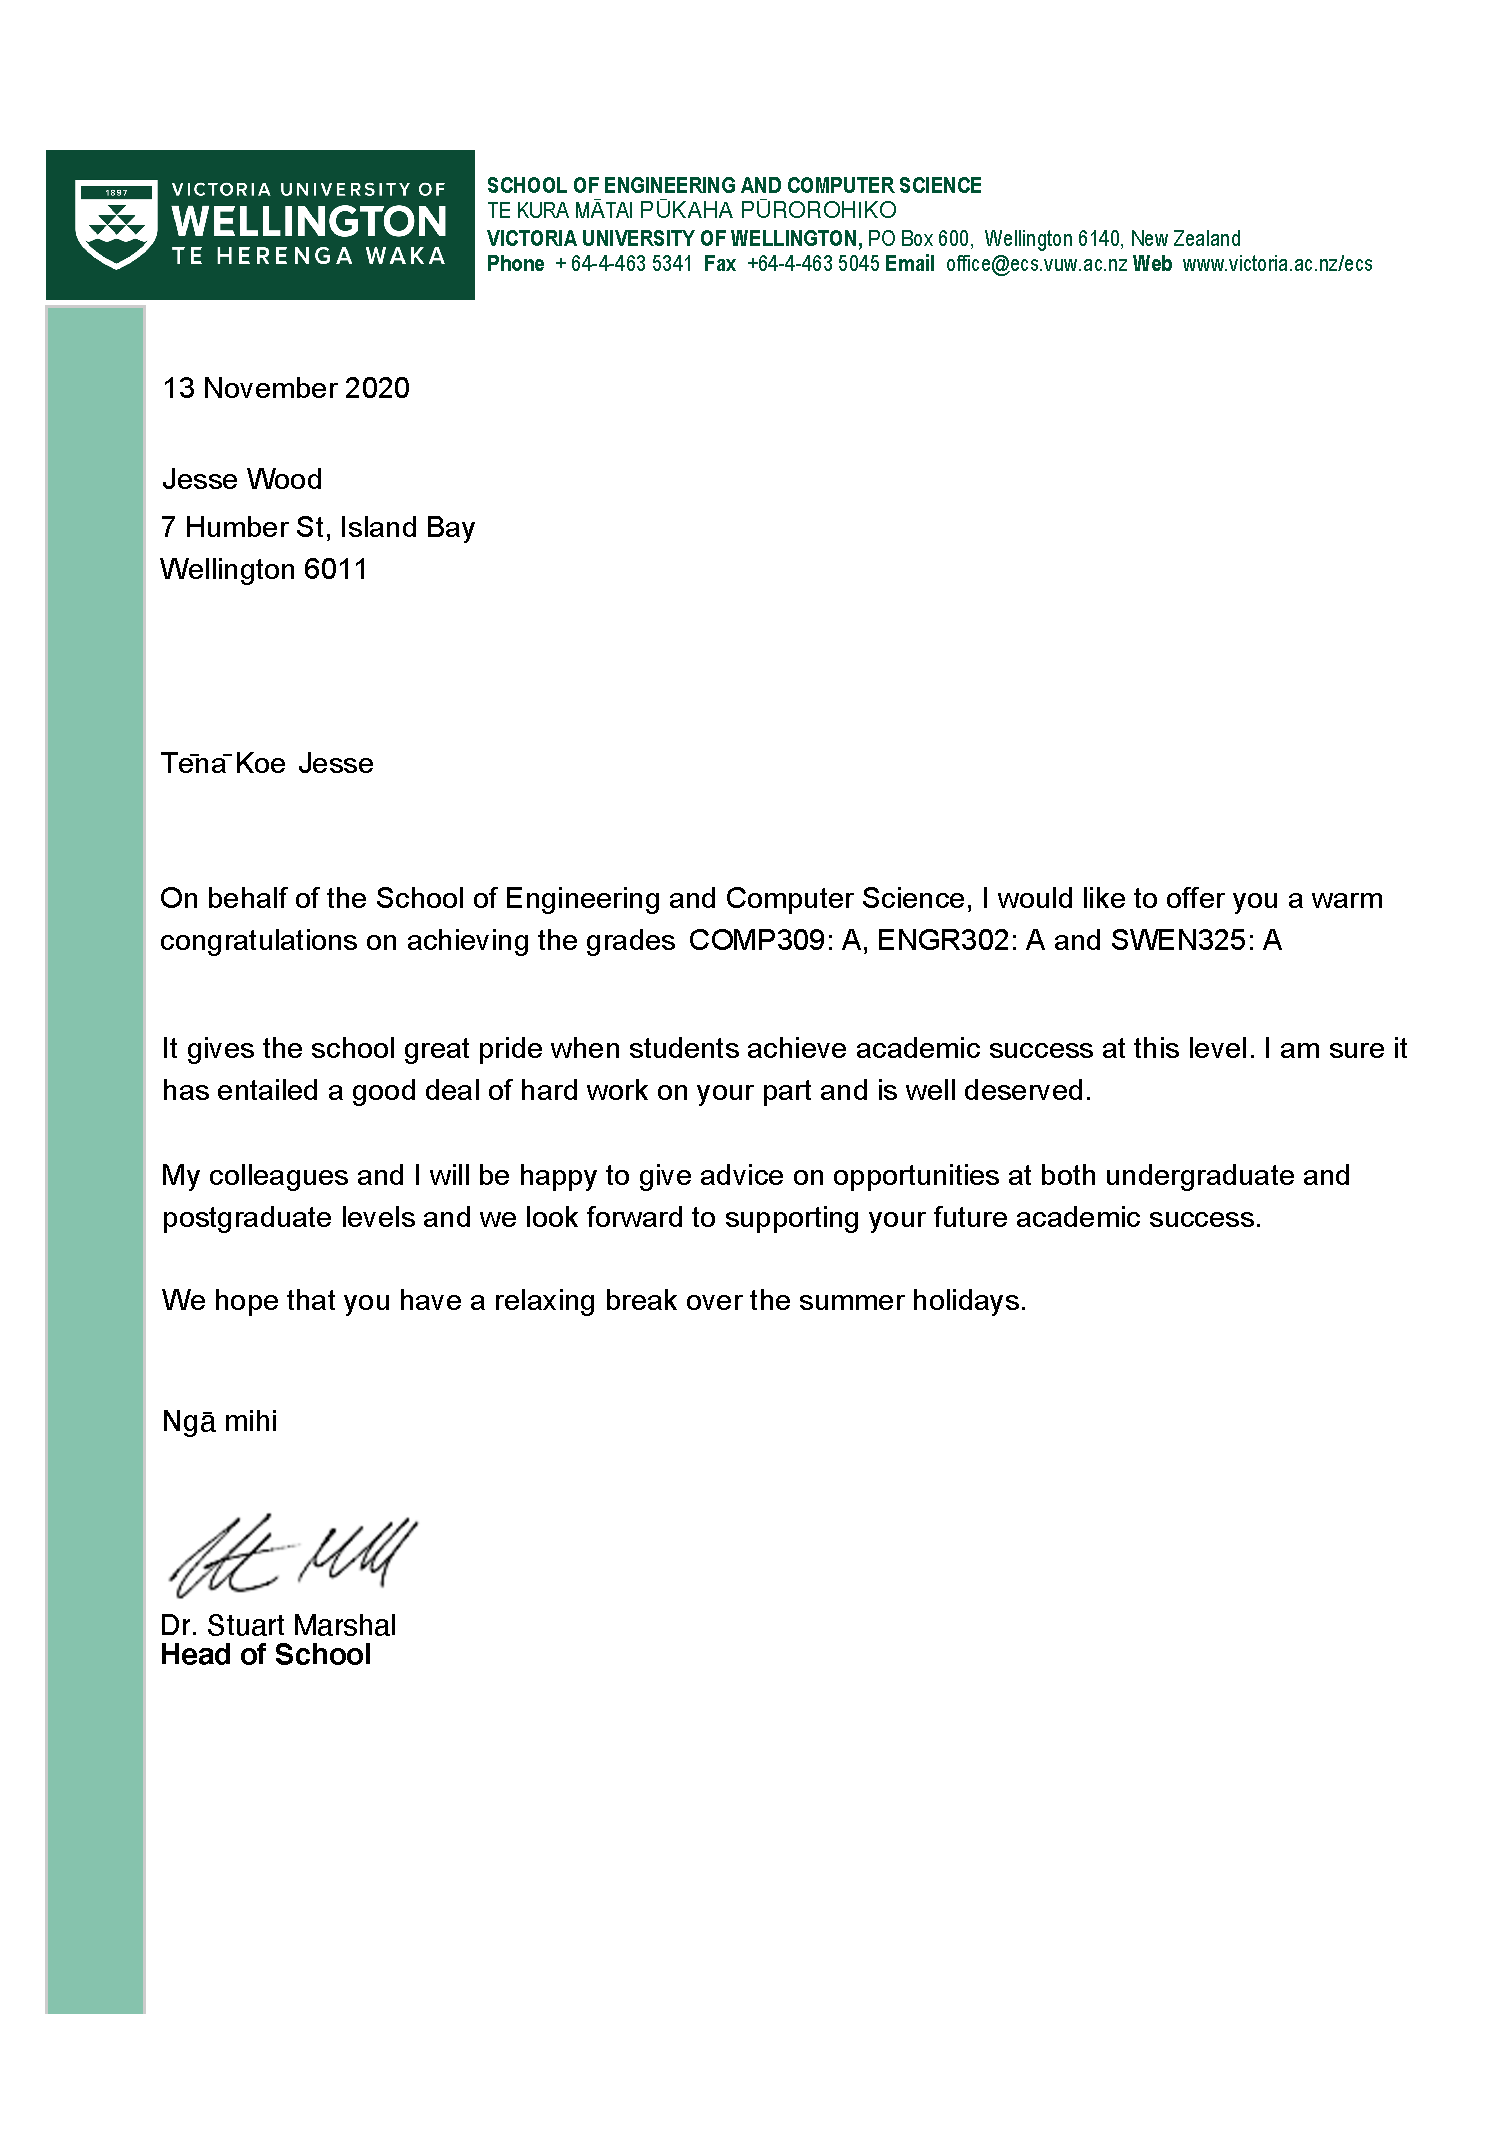
\includepdf[pages=-]{academic-certificate.pdf}

\end{document}
